\section{1174006 - Kadek Diva Krishna Murti}

\subsection{Teori}
\noindent
Jelaskan apa itu binary classification dilengkapi ilustrasi gambar sendiri.

\noindent
Binary Classification adalah jenis klasifikasi yang mengklasifikasikan elemen-elemen dari himpunan ke dalam dua kelompok berdasar aturan klasifikasi yang telah ditentukan. Contohnya : Spam Filtering

\hfill\break
\begin{figure}[H]
    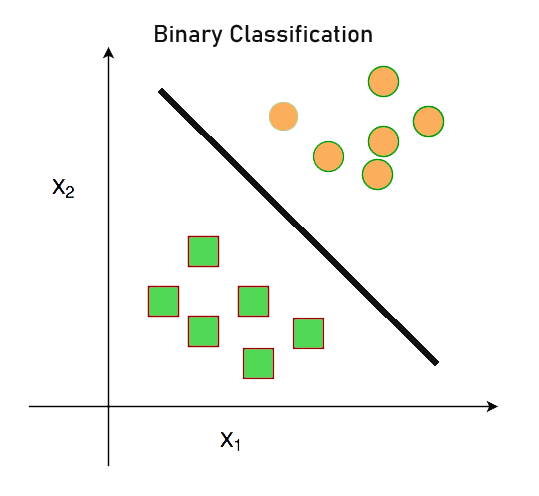
\includegraphics[width=1\textwidth]{figures/1174006/chapter2/teori/1.png}
    \centering
    \caption{Kecerdasan Buatan.}
\end{figure}

\noindent
Jelaskan apa itu supervised learning dan unsupervised learning dan clustering dengan ilustrasi gambar sendiri.

\noindent
Supervised Learning adalah pembelajaran yang memiliki label di tiap datanya. Label maksudnya adalah tag dari data yang ditambahkan dalam machine learning model. Contohnya gambar kucing di tag "kucing" di tiap masing masing image kucing dan gambar anjing di tag "anjing" di tiap masing gambar anjing.

\hfill\break
\begin{figure}[H]
    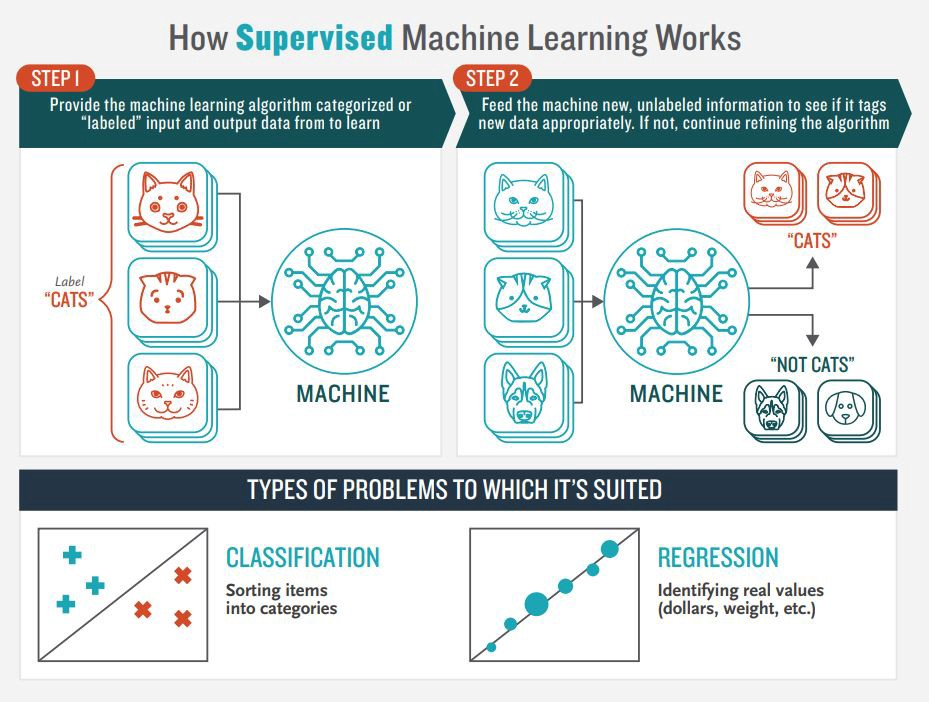
\includegraphics[width=1\textwidth]{figures/1174006/chapter2/teori/2.png}
    \centering
    \caption{Kecerdasan Buatan.}
\end{figure}

\noindent
Unsupervised learning adalah pemebelajaran yang tidak menggunakan label dalam memprediksi target feautures / variable. Melainkan menggunakan ke samaan dari attribut-attribut yang dimiliki. Jika attribut dan sifat-sifat dari data data feature yang diekstrak memiliki kemiripan, maka akan dikelompok kelompokan (clustering). Sehingga hal ini akan menimbulkan kelompok-kelompok (cluster).

\hfill\break
\begin{figure}[H]
    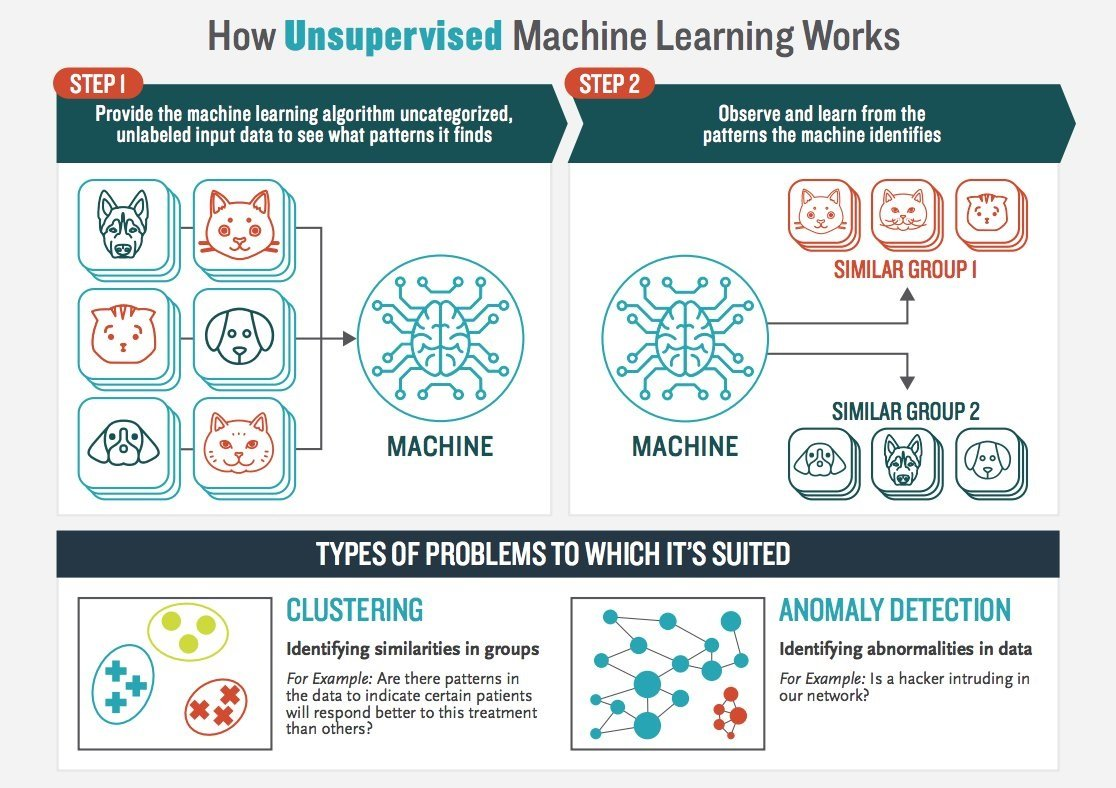
\includegraphics[width=1\textwidth]{figures/1174006/chapter2/teori/3.png}
    \centering
    \caption{Kecerdasan Buatan.}
\end{figure}

\noindent
Clustering adalah  metode untuk mengelompokan data-data menjadi kumpulan grup yang isinya merupakan data yang serupa dengan grupnya. Basisnya dapat berupa kesamaan atau perbedaan dari setiap grup tersebut.

\hfill\break
\begin{figure}[H]
    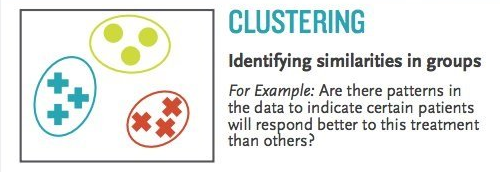
\includegraphics[width=1\textwidth]{figures/1174006/chapter2/teori/4.png}
    \centering
    \caption{Kecerdasan Buatan.}
\end{figure}

\noindent
Jelaskan  apa  itu  evaluasi  dan  akurasi  dari  buku  dan  disertai  ilustrasi  contoh dengan gambar sendiri.

\noindent
Evaluasi adalah bagaimana kita dapat mengevaluasi seberapa baik model bekerja dengan cara mengukur akurasinya. Dan akurasi adalah seberapa benar persentase pemebelajaran dengan kasus yang diklasifikasikan. 

\noindent
Kita dapat menganalisis kesalahan yang dibuat oleh model, atau tingkat kebingungannya, menggunakan matriks kebingungan (confusion matrix). Matriks kebingungan mengacu pada kebingungan dalam model, tetapi matriks kebingungan ini bisa menjadi sedikit sulit untuk dipahami ketika mereka menjadi sangat besar.

\hfill\break
\begin{figure}[H]
    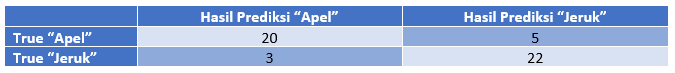
\includegraphics[width=1\textwidth]{figures/1174006/chapter2/teori/5.png}
    \centering
    \caption{Kecerdasan Buatan.}
\end{figure}

\noindent
Jelaskan bagaimana cara membuat dan membaca confusion matrix, buat confusion matrix buatan sendiri.

\noindent
Confusion Matrix merupakan metode untuk menghitung akurasi pada model. Confusion Matrix merepresentasikan prediksi dan kondisi sebenarnya(aktual) dari data yang dihasilkan oleh algoritma ML. Berdasarkan Confusion Matrix, kita bisa menentukan Accuracy, Precission, Recall dan Specificity. Pada pengukuran kinerja menggunakan confusion matrix, terdapat 4 (empat) istilah sebagai representasi hasil proses klasifikasi, diantaranya adalah :
\begin{itemize}
    \item True Positive : Data positif yang terdeteksi memiliki hasil benar
    \item False Positive : Data Positif yang terdeteksi memiliki hasil salah
    \item True Negative : Data negatif yang terdeteksi memiliki hasil benar
    \item False Negative : Data negatif yang terdeteksi memiliki hasil salah
\end{itemize}

\hfill\break
\begin{figure}[H]
    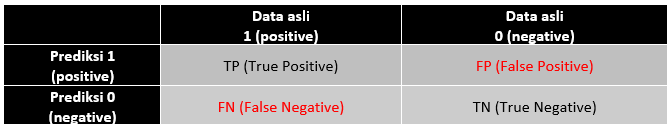
\includegraphics[width=1\textwidth]{figures/1174006/chapter2/teori/6.png}
    \centering
    \caption{Kecerdasan Buatan.}
\end{figure}

\noindent
Jelaskan  bagaimana  K-fold  cross  validation  bekerja  dengan  gambar  ilustrasi contoh buatan sendiri.

\noindent
Cara kerja k-fold validation:
\begin{itemize}
	\item Total instance dibagi menjadi N bagian.
	\item Fold yang pertama adalah bagian pertama menjadi data uji (testing data) dan sisanya menjadi training data.
	\item Lalu hitung akurasi berdasarkan porsi data tersebut dengan menggunakan persamaan.
	\item Fold yang kedua adalah bagian kedua, yang menjadi data uji(testing data)dan sisanya training  data.
	\item Kemudian hitung akurasi berdasarkan porsi data tersebut.
	\item Dan seterusnya hingga habis mencapai fold ke-K.
	\item Terakhir hitung rata-rata akurasi K buah.
\end{itemize}

\hfill\break
\begin{figure}[H]
    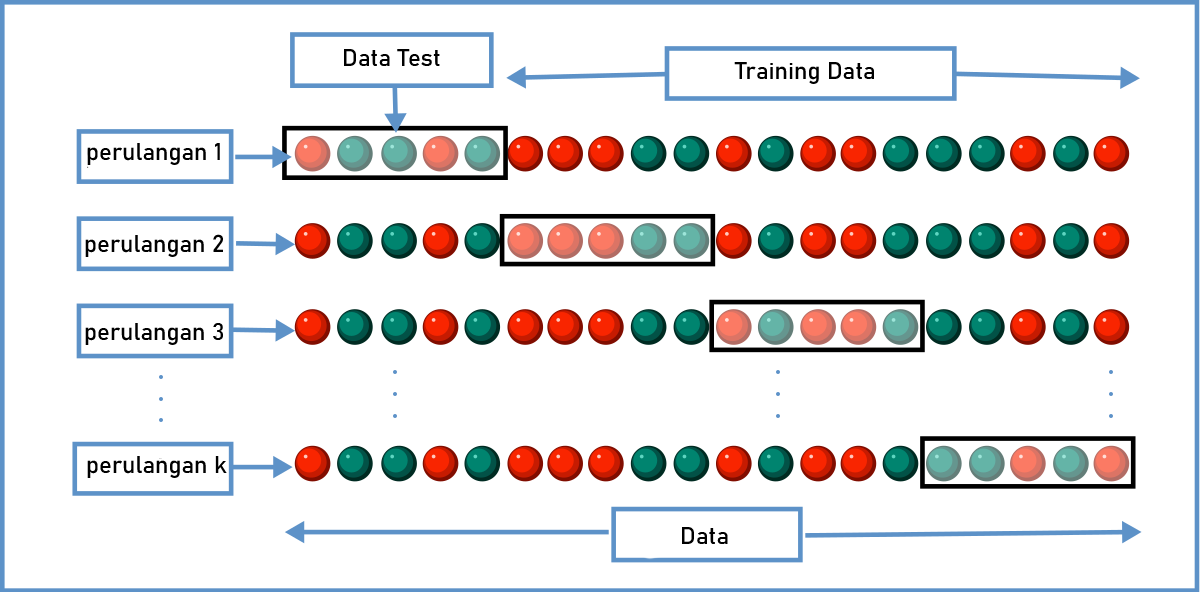
\includegraphics[width=1\textwidth]{figures/1174006/chapter2/teori/7.png}
    \centering
    \caption{Kecerdasan Buatan.}
\end{figure}

\noindent
Jelaskan apa itu decision tree dengan gambar ilustrasi contoh buatan sendiri.

\noindent
Decision Tree merupakan sebuah struktur yang menentukan keputusan dan setiap konsekuensinya. Hasil dari setiap struktur biasanya menggunakan jawaban (True dan False) atau cabang lain yang akan menjadi pohon selanjutnya. Setiap keputusan diantaranya akan membandingkan kondisi yang diberikan kepada struktur untuk dibandingkan kondisi apa saja yang sudah didapat pada sistem tersebut.

\hfill\break
\begin{figure}[H]
    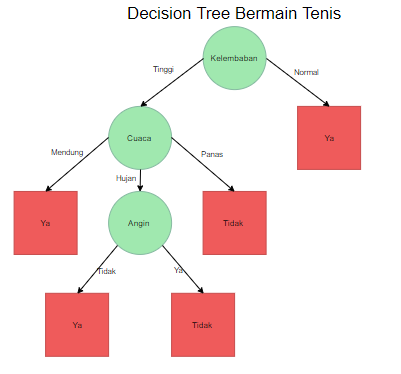
\includegraphics[width=1\textwidth]{figures/1174006/chapter2/teori/8.png}
    \centering
    \caption{Kecerdasan Buatan.}
\end{figure}

\noindent
Jelaskan apa itu information gain dan entropi dengan gambar ilustrasi buatan sendiri.

\noindent
Information Gain merupakan total data yang didapat dari data - data acak yang data tersebut akan digunakan untuk analisis data lainnya. Information Gain ini digunakan pada decision tree sebagai label setiap aksi - aksi yang perlu dinilai validasinya.

\hfill\break
\begin{figure}[H]
    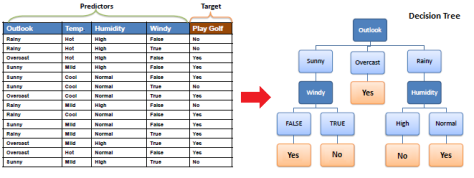
\includegraphics[width=1\textwidth]{figures/1174006/chapter2/teori/9.png}
    \centering
    \caption{Kecerdasan Buatan.}
\end{figure}

\noindent
Entropi merupakan pengukuran sebuah data dan validnya data tersebut untuk dapat digunakan sebagai informasi yang akan dimasukkan ke Information Gain. Entropi menilai sebuah obyek berdasarkan kebutuhan di dunia nyata dan pengaruh pada sistem yang akan digunakan.

\hfill\break
\begin{figure}[H]
    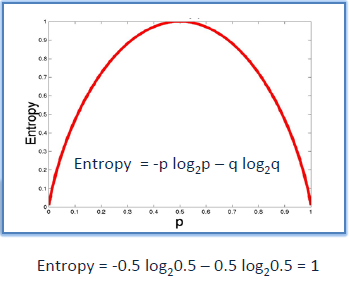
\includegraphics[width=1\textwidth]{figures/1174006/chapter2/teori/10.png}
    \centering
    \caption{Kecerdasan Buatan.}
\end{figure}

\subsection{Praktek}

\lstinputlisting[firstline=4, lastline=9]{src/1174006/chapter2/1174006.py}
\hfill\break
\begin{figure}[H]
    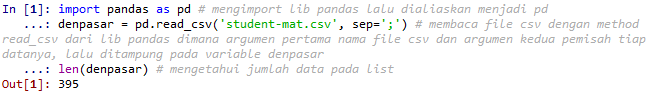
\includegraphics[width=1\textwidth]{figures/1174006/chapter2/praktek/1.png}
    \centering
    \caption{Kecerdasan Buatan.}
\end{figure}

\lstinputlisting[firstline=10, lastline=15]{src/1174006/chapter2/1174006.py}
\hfill\break
\begin{figure}[H]
    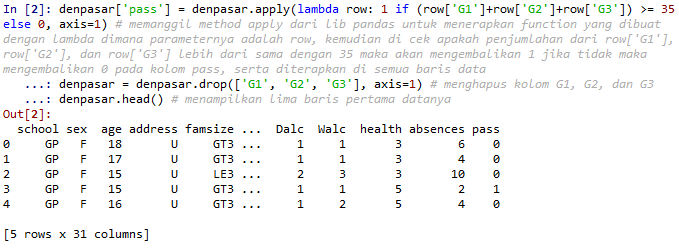
\includegraphics[width=1\textwidth]{figures/1174006/chapter2/praktek/2.png}
    \centering
    \caption{Kecerdasan Buatan.}
\end{figure}

\lstinputlisting[firstline=17, lastline=20]{src/1174006/chapter2/1174006.py}
\hfill\break
\begin{figure}[H]
    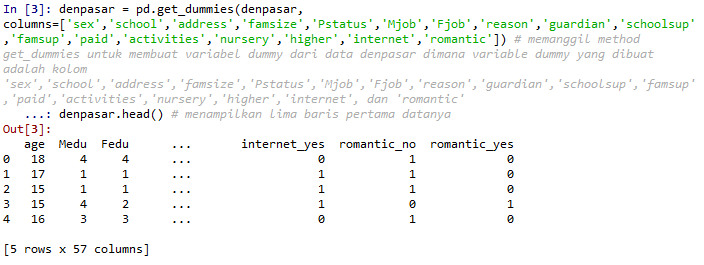
\includegraphics[width=1\textwidth]{figures/1174006/chapter2/praktek/3.png}
    \centering
    \caption{Kecerdasan Buatan.}
\end{figure}

\lstinputlisting[firstline=22, lastline=40]{src/1174006/chapter2/1174006.py}
\hfill\break
\begin{figure}[H]
    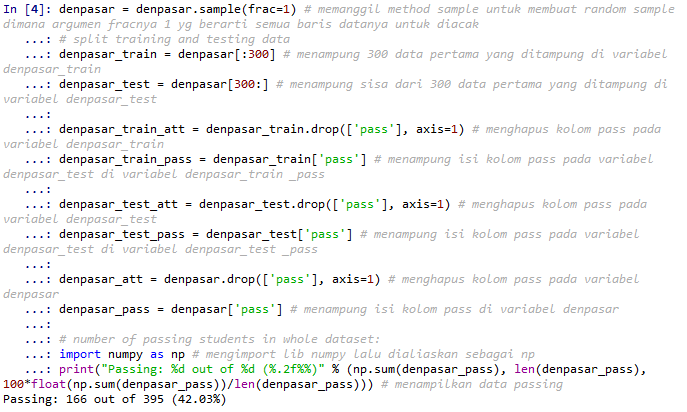
\includegraphics[width=1\textwidth]{figures/1174006/chapter2/praktek/4.png}
    \centering
    \caption{Kecerdasan Buatan.}
\end{figure}

\lstinputlisting[firstline=42, lastline=46]{src/1174006/chapter2/1174006.py}
\hfill\break
\begin{figure}[H]
    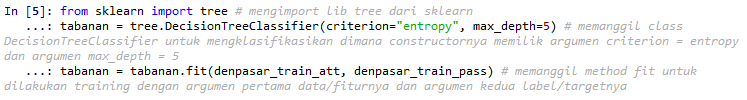
\includegraphics[width=1\textwidth]{figures/1174006/chapter2/praktek/5.png}
    \centering
    \caption{Kecerdasan Buatan.}
\end{figure}

\lstinputlisting[firstline=48, lastline=53]{src/1174006/chapter2/1174006.py}
\hfill\break
\begin{figure}[H]
    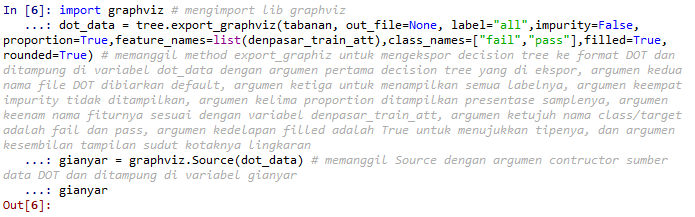
\includegraphics[width=1\textwidth]{figures/1174006/chapter2/praktek/6-1.png}
    \centering
    \caption{Kecerdasan Buatan.}
\end{figure}
\hfill\break
\begin{figure}[H]
    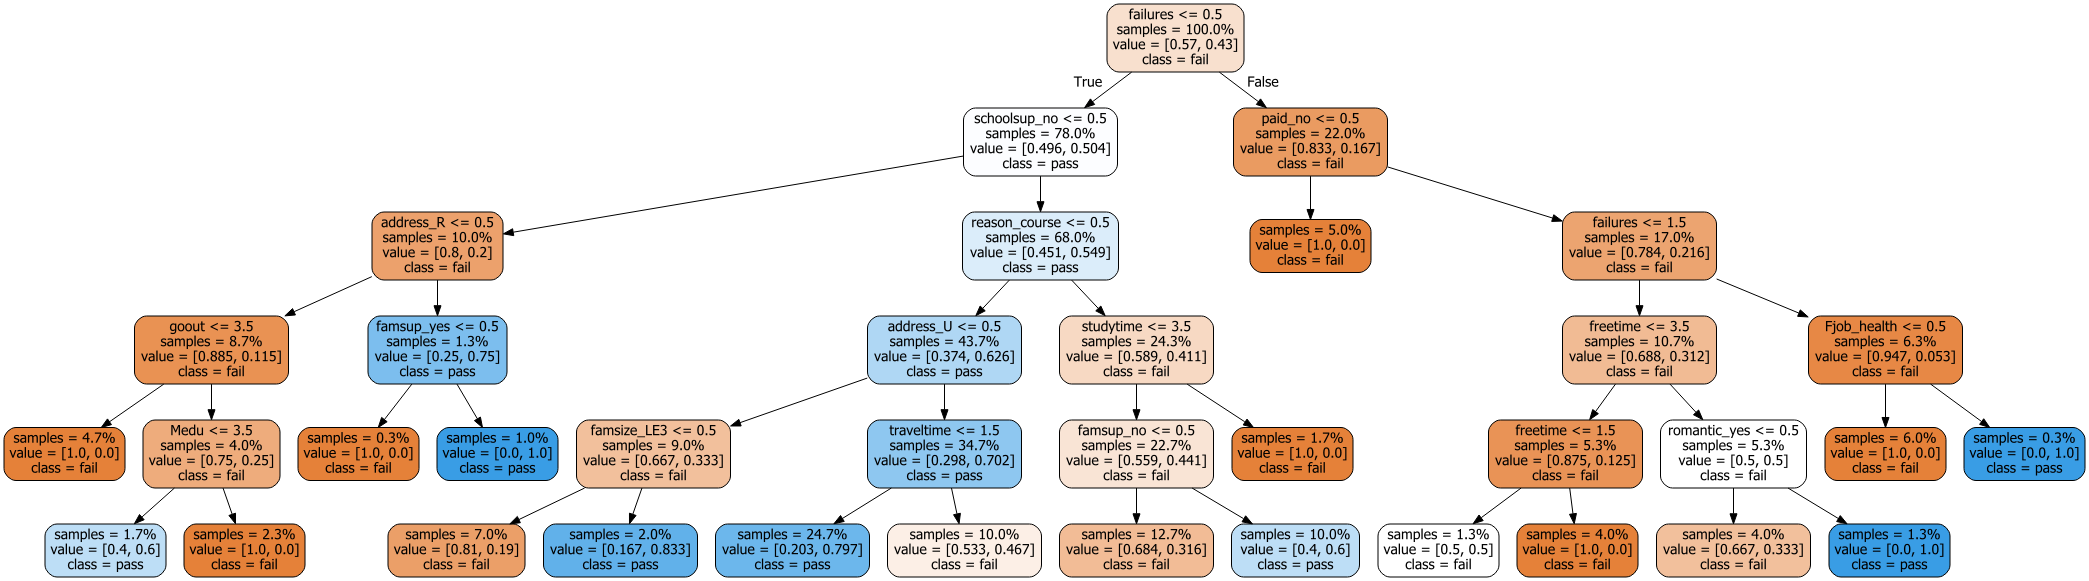
\includegraphics[width=1\textwidth]{figures/1174006/chapter2/praktek/6-2.png}
    \centering
    \caption{Kecerdasan Buatan.}
\end{figure}

\lstinputlisting[firstline=55, lastline=57]{src/1174006/chapter2/1174006.py}
\hfill\break
\begin{figure}[H]
    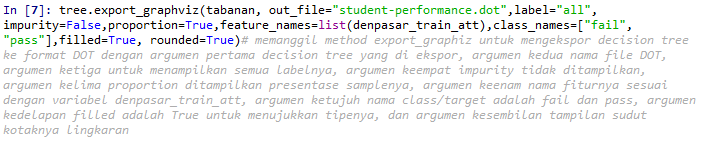
\includegraphics[width=1\textwidth]{figures/1174006/chapter2/praktek/7.png}
    \centering
    \caption{Kecerdasan Buatan.}
\end{figure}

\lstinputlisting[firstline=59, lastline=60]{src/1174006/chapter2/1174006.py}
\hfill\break
\begin{figure}[H]
    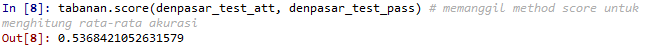
\includegraphics[width=1\textwidth]{figures/1174006/chapter2/praktek/8.png}
    \centering
    \caption{Kecerdasan Buatan.}
\end{figure}

\lstinputlisting[firstline=62, lastline=67]{src/1174006/chapter2/1174006.py}
\hfill\break
\begin{figure}[H]
    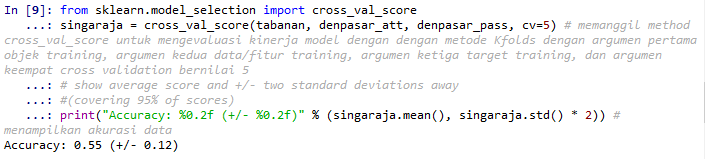
\includegraphics[width=1\textwidth]{figures/1174006/chapter2/praktek/9.png}
    \centering
    \caption{Kecerdasan Buatan.}
\end{figure}

\lstinputlisting[firstline=69, lastline=73]{src/1174006/chapter2/1174006.py}
\hfill\break
\begin{figure}[H]
    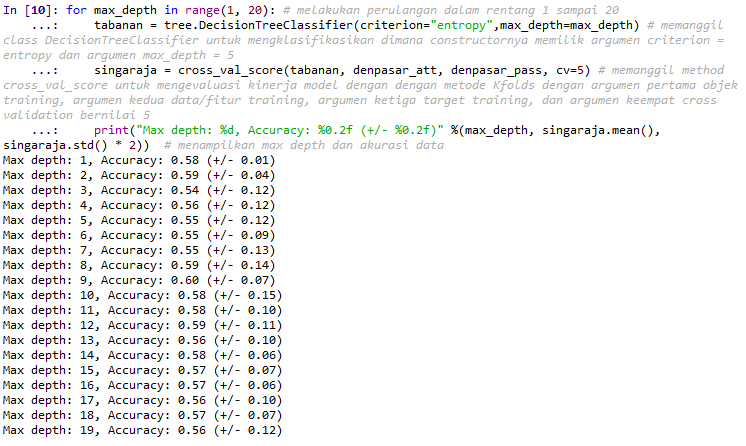
\includegraphics[width=1\textwidth]{figures/1174006/chapter2/praktek/10.png}
    \centering
    \caption{Kecerdasan Buatan.}
\end{figure}

\lstinputlisting[firstline=75, lastline=86]{src/1174006/chapter2/1174006.py}
\hfill\break
\begin{figure}[H]
    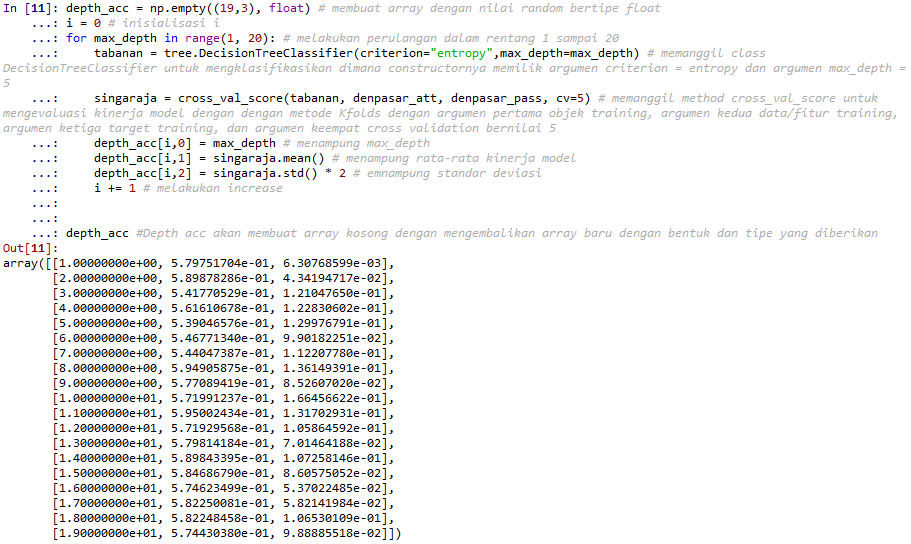
\includegraphics[width=1\textwidth]{figures/1174006/chapter2/praktek/11.png}
    \centering
    \caption{Kecerdasan Buatan.}
\end{figure}

\lstinputlisting[firstline=88, lastline=92]{src/1174006/chapter2/1174006.py}
\hfill\break
\begin{figure}[H]
    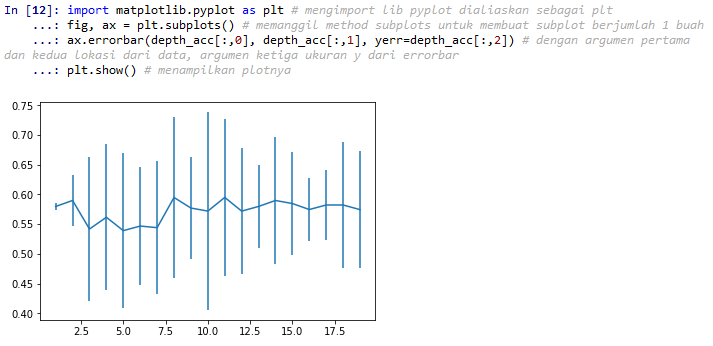
\includegraphics[width=1\textwidth]{figures/1174006/chapter2/praktek/12.png}
    \centering
    \caption{Kecerdasan Buatan.}
\end{figure}

\subsection{Penanganan Error}
\begin{enumerate}
	\item Skrinsut error.
	\begin{itemize}
		\item Name Error
		\hfill\break
		\begin{figure}[H]
			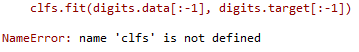
\includegraphics[width=1\textwidth]{figures/1174006/chapter1/error/err3.PNG}
			\centering
			\caption{Name Error.}
		\end{figure}
		\item Import Error
		\hfill\break
		\begin{figure}[H]
			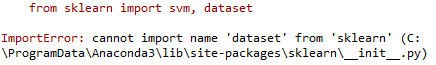
\includegraphics[width=1\textwidth]{figures/1174006/chapter1/error/err1.PNG}
			\centering
			\caption{Import Error.}
		\end{figure}
		\item Value Error
		\hfill\break
		\begin{figure}[H]
			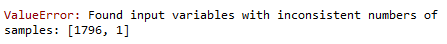
\includegraphics[width=1\textwidth]{figures/1174006/chapter1/error/err2.PNG}
			\centering
			\caption{Value Error.}
		\end{figure}
		\item Syntax Error
		\hfill\break
		\begin{figure}[H]
			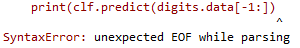
\includegraphics[width=1\textwidth]{figures/1174006/chapter1/error/err4.PNG}
			\centering
			\caption{Syntax Error.}
		\end{figure}
	\end{itemize}
	\item Tuliskan kode eror dan jenis errornya.
	\begin{itemize}
		\item Name Error
		\hfill\break
		Name Error adalah exception yang terjadi saat syntax melakukan eksekusi terhadap local name atau global name yang tidak terdefinisi.
		\item Import Error
		\hfill\break
		Import Error adalah exception yang terjadi saat syntax melakukan import terhadap library yang tidak terdefinisi.
		\item Value Error
		\hfill\break
		Value Error adalah exception yang terjadi saat syntax memiliki nilai yang tidak valid.
		\item Syntax Error
		\hfill\break
		Syntax Error adalah exception yang terjadi saat ada kesalahan dalam mengetikkan syntax.
	\end{itemize}
	\item Solusi pemecahan masalah error tersebut.
	\begin{itemize}
		\item Name Error
		\hfill\break
		Solusinya adalah memastikan variabel atau function yang dipanggil ada atau tidak salah ketik.
		\item Import Error
		\hfill\break
		Solusinya adalah memastikan library yang dipanggil ada atau tidak salah ketik.
		\item Value Error
		\hfill\break
		Solusinya adalah memastikan nilai yang diinputkan valid.
		\item Syntax Error
		\hfill\break
		Solusinya adalah memastikan syntax yang diketik tidak salah ketik.
	\end{itemize}
\end{enumerate}

\subsection{Bukti Tidak Plagiat}
\begin{figure}[H]
	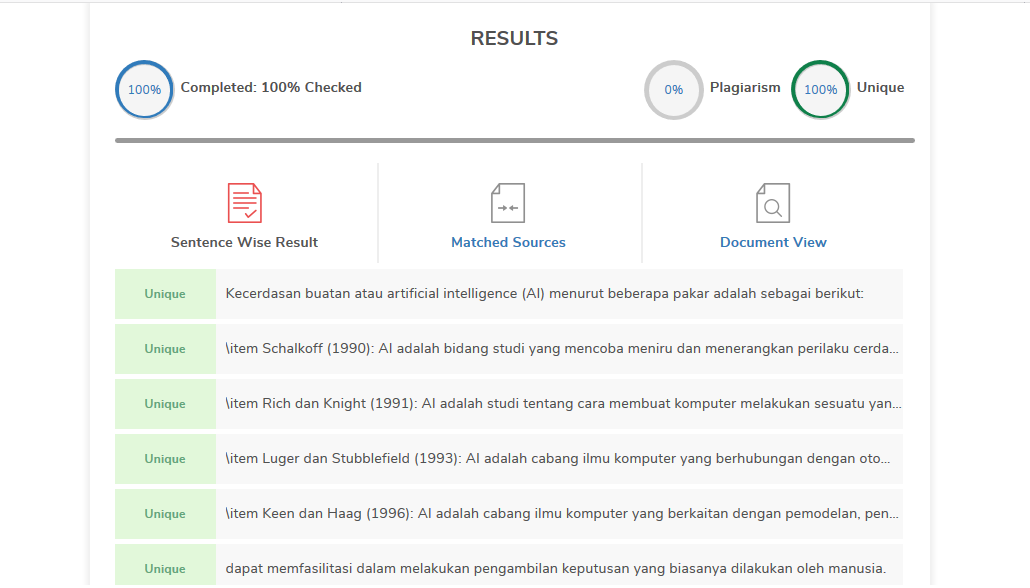
\includegraphics[width=1\textwidth]{figures/1174006/chapter1/plagiat.png}
	\centering
	\caption{Bukti Tidak Plagiat.}
\end{figure}